\section{Problem  formulation}
\label{sec:problem}

According to the World Health Organization (WHO), heart disease is 
the leading cause of death around the world.
More than $1000$ Americans died each day in $2016$ from heart 
attacks. 
Although a single arrhythmia heartbeat will not have a serious impact 
on life, continuous arrhythmia can result in fatal circumstances.
For instance, \textit{Ventricular Tachycardia} (VT) is a potentially 
fatal arrhythmia. 
% caused by abnormal electrical signals in the lower chambers of the 
%heart (ventricles).
On the other hand, \textit{Supraventricular Tachycardia} (SVT)
is not considered to be dangerous for most of people. 
% originates in the upper part of the heart (atria). 

The problem we decided to work on is cardiac arrhythmias 
discrimination. We view this problem as a binary classification task 
that discriminates whether a patient has VT (fatal tachycardia) or  
SVT (non-fatal tachycardia). The will analyze, implement and compare 
four classification algorithms: DNN, SVM (with and without 
PCA), 
decision tree and \knn.


%The first step of many algorithms that we will implement is feature 
%extraction. For ECG signals, those features can include, but not 
%limited to: signal amplitude, beat duration, signal segments and 
%waves durations, frequency domain features, short beats counter. 
%We plan to use cross-validation to find the optimal set of features.

We will use the following performance measures:
\begin{itemize}
	\item Precision, 
	%sensitivity or 
	TPR ($\#$ correctly detected VT/$\#$ true VTs), 
	%specificity or 
	TNT ($\#$ correctly detected SVT/$\#$ true SVTs). 
	Those are very important performance measures in case of 
	tachycardia discrimination. Though FP (misclassifying SVT as VT) 
	might lead 	to a 	process of further examination or treatment 
	episodes which are 
	painful for the patient, FN (misclassifying VT as SVT) might put 
	the patient in the risk of death.  
%	Due to this reason, using cost sensitive loss is another possible 
%	approach we will use.
	\item For DNN and SVM with PCA performance we will also measure 
	training 
	and test time.
	\item Since PCA is used to reduce calculation costs, we will 
	specifically 
	measure how much training time was reduced after using PCA while 
	test error is still above threshold. 
	\item Since \knn is a memory-based algorithm we will report its 
	test times. 
\end{itemize}


%\begin{figure*}[t]
%	\centering
%	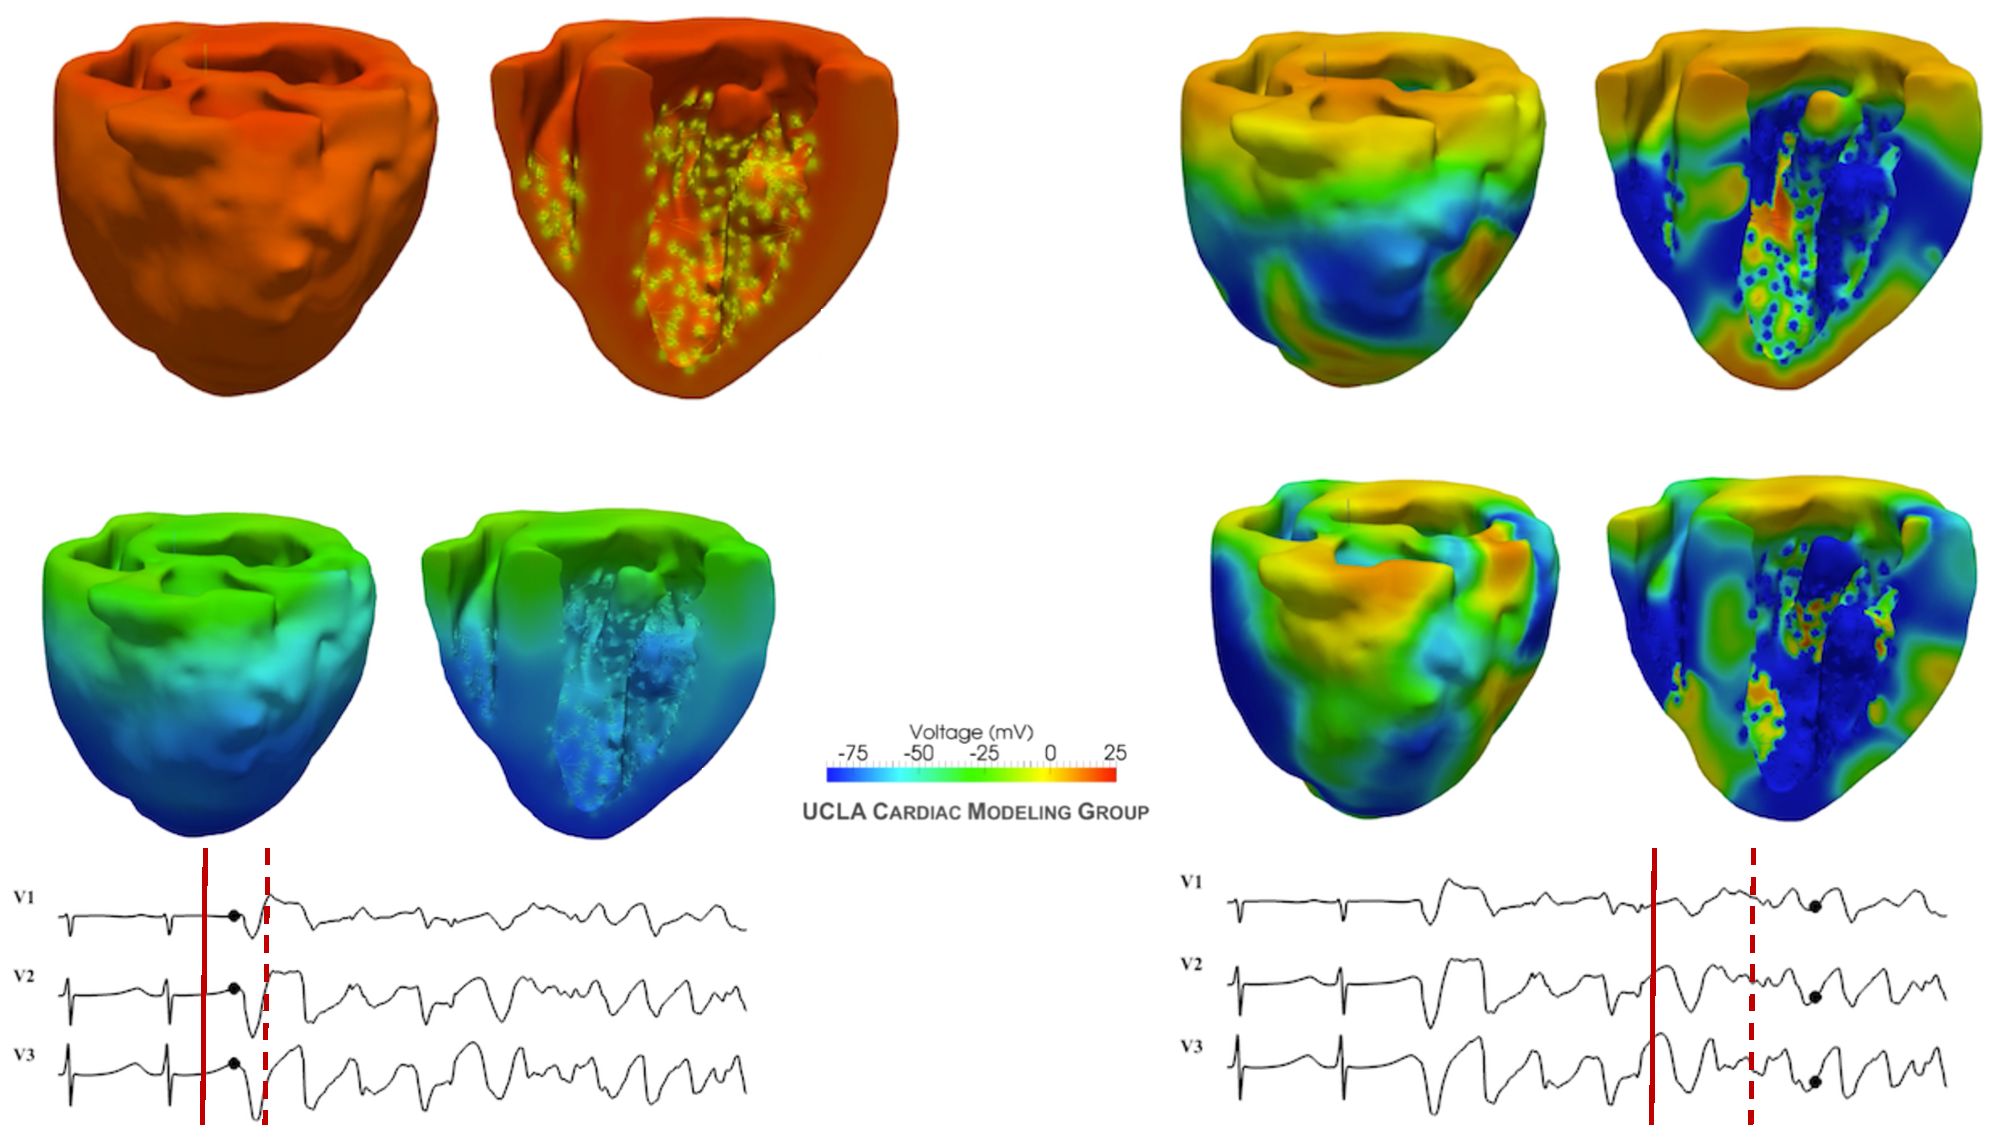
\includegraphics[width=0.9\linewidth]{figures/whnsrvfLowres.pdf}
%	\caption{Electrical activity during NSR and VF. The 
%	color scale runs from blue = rest state to red = excited (aka 
%	depolarized) state. (Colors in digital version).
%		In the top left, the ventricles are shown from two different 
%		angles, during a phase of NSR. The ventricles are fully 
%		exicted. The bottom left panel shows a later phase of the 
%		same beat, where the ventricles are progressively relaxing, 
%		starting with the apex (the pointed tip of the heart). This 
%		orderly propagation insures adequate muscle contraction and 
%		blood flow.
%		Three surface ECGs are shown beneath the left column, with 
%		red bars indicating the timing of the two snapshots. Note the 
%		periodic pattern.
%		The right column shows two snapshots during VF (earlier 
%		snapshot on top).
%		Note the disorganized nature of the electrical activity, 
%		wavefront breakup, and the multiple regions of 
%		depolarization. Note also the change in the surface ECG from 
%		periodic and regular (early on) to disorganized.
%		The AMA reads two such signals (obtained, however, 
%		intra-cardially and not from the surface) and tries to detect 
%		fibrillation. [Obtained from video of a simulation of the 
%		ventricles by the UCLA Cardiac Modeling Group, courtesy of 
%		Luigi Perrotti]}
%	\label{fig:whnsrvf}
%\end{figure*}